\documentclass{iarticle}
\usepackage{ctex}
\usepackage{imath}

\title{基于多元回归模型对住房价格的预测与影响因素分析}
\author{李泽宇, 李钦, 陈奕玮}
% \date{}

\bibliographystyle{acm}

\begin{document}
\begin{center}
  \vspace*{1cm}

  \Huge
  \textbf{基于多元回归模型对住房价格的预测与影响因素分析}

  \vspace{0.5cm}
  \LARGE
  \textbf{}

  \vspace{1.5cm}

  \begin{tabular}{rll}
    \textbf{李钦}   & \textbf{2020012872} & \textbf{未央-水木 02} \\
    \textbf{李泽宇} & \textbf{2020012879} & \textbf{未央-水木 02} \\
    \textbf{陈奕玮} & \textbf{2020012881} & \textbf{未央-水木 02} \\
  \end{tabular}

  \vspace{1cm}

  \textbf{指导教师: \quad 吴璟}

  \vfill

  \textbf{Engineering Economy}

  \vspace{0.8cm}

  \includegraphics[width=0.4\textwidth]{/mnt/d/images/Tsinghua_University_Logo.png}

  \Large
  \textbf{Weiyang College}

  \textbf{Tsinghua University}

  \textbf{}

  \textbf{\today}

\end{center}
\newpage

\begin{abstract}
  房价问题一直以来都是百姓关注的热门话题.
  作为国家的支柱产业之一, 房价的走势与区域经济的发展常常有着密不可分的联系.
  在城市元素日益多样化, 商品住房因金融属性的增加而呈现较大的不确定性的今天, 影响房价的相关因素的分析显得尤为重要.
  本研究着眼于住房周边的地点, 探究住房周边设施, 场所等区位因素及其距离远近对于住房价格的影响, 并根据建立的简单模型进行拟合, 取得较为良好的估测效果.

  本项目已在 \url{https://github.com/godvix/housing-price-model} 开源.

  \paragraph{关键词:}
  住房价格; 多元回归分析; POI
\end{abstract}

\tableofcontents
\listoffigures
\listoftables

% !TeX root = main.tex
\section{引言}
房价问题一直以来都是百姓关注的热门话题.
作为国家的支柱产业之一, 房地产的走势常常能够影响到区域经济的发展.
近年来不断走高的房价, 不断膨胀的房地产泡沫令人担忧.
但是, 住房的真实价值却一直是一个未知数.
在不同人眼中, 住房的价值可能完全不同.
但对于消费市场而言, 住房的真实价值应当是相对确定的.
通过分析住房价格的影响因素能够一定程度上确定商品房的市场价格中金融属性所占的比重.

现有住房价格影响因素的分析往往基于居民收入, 税收政策等宏观因素, 或基于交通设施等单一因素.
住房价格通常与周边诸多环境, 基础设施等高度相关, 而不仅仅只与单一因素相关.
如果能够量化这种多元相关性, 住房价格的空间分布能够在一定程度上表征城市居民对住房周边设施所带来的效益的支付意愿, 这将能够作为评价支付意愿的重要依据之一, 有利于计算难以量化的外部性的影子价格.
此外, 通过引入更加全面的影响因素, 可能可以识别出城市的特征, 发现不同城市间的偏好差异.

在课堂上, 老师介绍了市场分析中的回归分析法.
回归分析法可以通过输入数据, 得到一系列自变量对于因变量的影响因子, 给出不同自变量对于因变量的影响程度大小;同时, 这种影响因子的结果也有助于预测一定自变量条件下因变量的值.

这样的模型可以通过考虑交通便捷性对于房价的影响来估算人们对于通勤时间的支付意愿, 从而计算地铁的社会总效益.
经过思考后与阅读文献后, 本文拟采用回归分析法来对房价的影响因素进行分析, 得到因素对于房价的作用因子;得到影响因子后, 本文借助该模型对于房价进行预测.

% !TeX root = main.tex
\section{相关工作}
在研究某一地区住房价格影响因素的过程中, 许多研究者采用回归分析法, GWR 模型法等方法进行研究.
由于本文的模型是考虑区位对房价的影响情况, 本部分主要关注那些采用区位的视角来考察房价的研究.
西南大学的刘青霞, 王方民两人在其硕士论文中都利用了回归分析法对某个特定的因素对于房价的影响做了估计. \cite{RN4,RN5}

阅读文章, 可以发现刘青霞建立的模型在一些方面合理且细致, 但不难发现, 研究的结果并不如人意.
例如, 我们发现刘青霞的回归分析模型 $R^2$ 只有 \num{0.5415}, 可以发现, 这一方面显然来源于其模型的过度简化.

在刘的研究中, 对于所有的影响因素, 都统一取了该居民小区到距离其最近的该类建筑的距离, 而这种过度的简化其实是不合理的.
首先, ``取最小值'' 的方法本身对于某些影响因素是不合理的.
例如, 在研究中, 作者对于居民建筑与所有火车站之间的距离取最小值.
然而, 无论是在大家购买房子的时候, 还是在实际使用的过程中, 居民实际前往哪一个火车站是基于特定列车的始发车站的, 与``最近的火车站距离'' 其实没有直接关系.
其次, ``取最小值'' 的处理就导致在其研究中, 所有的模型在组内都是不分排名, 不加权重的.
比如, 在模型中所有的轨道交通站都是一致的.
然而, 在现实生活中, 多条线路交汇的轨道交通站与只有一条线路的轨道交通站对于周围房价的影响一定是有不同的.

对于以上两个方面, 如果模型如果能改成对于一定区域内的轨交车站, 火车站按照其重要性取加权平均, 那么就会显得更加合理.

% !TeX root = main.tex
\section{模型选择}
受限于专业知识的不足, 本研究选用较为简单的模型作为示例进行分析.

假设住房价格受到工业, 教育, 商业, 医疗, 交通, 旅游等周边因素的影响, 影响程度与住房与周边重要区位中心的距离有关.
简单起见, 本研究选用直线距离作为权重, 选取若干企业, 学校, 商业中心, 医院, 交通枢纽, 作为 POI (Point of Interest), 可以得到住房与这些 POI 之间的直线距离.

对于不同的 POI, 其影响力必然不同.
假设选取的所有 POI 的影响范围 ($Scope$) 从 $e^3$, 按排名, 指数递减至 $e^{-3}$.
考虑某个 $poi$, 其对房价的影响为
\begin{equation*}
    \delta\ipp{Price} = \exp\iBB{-\frac{Dist\ibb{poi}}{Scope\ibb{poi}}}
\end{equation*}
其中 $Dist\ibb{poi}$ 表示住房与该 POI 之间的直线距离.
住房的价格近似满足
\begin{equation*}
    Price
    = \sum_{category} \ipp{Impact\ibb{category} * \sum_{poi} \exp\iBB{-\frac{Dist\ibb{poi}}{Scope\ibb{poi}}}}
\end{equation*}

通过回归计算可以得到相应的系数 $Impact\ibb{category}$, 这表征着该类 POI 对于房价的影响程度.

% !TeX root = main.tex
\section{数据来源}
为了对房价的区位因素进行分析, 本研究需要北京与上海两地各个小区房价, 各类设施位置与排名两方面数据.
对于两地各小区房价, 采用网络上的两地2018年的各小区房价信息, 如图 \ref{fig:housing} 所示.

\begin{figure}[H]
  \centering
  \subcaptionbox{北京市}{\includegraphics[width=.45\linewidth]{figures/beijing_housing.png}}
  \subcaptionbox{上海市}{\includegraphics[width=.45\linewidth]{figures/shanghai_housing.png}}
  \caption{住房价格样本分布}
  \label{fig:housing}
\end{figure}

对于两地各类设施位置, 利用高德地图的POI搜索功能, 能够获取两地地图上的全部设施的信息, 如图 \ref{fig:poi} 所示.

\begin{figure}[H]
  \centering
  \subcaptionbox{北京市}{\includegraphics[width=.45\linewidth]{figures/beijing_poi.png}}
  \subcaptionbox{上海市}{\includegraphics[width=.45\linewidth]{figures/shanghai_poi.png}}
  \caption{POI 分布}
  \label{fig:poi}
\end{figure}

令人惊喜的是, 所有的设施已经被高德开放平台划入了一定的类别.
基于本文研究目标, 本文对高德开放平台分类进行了一些调整: 对一些类别进行了合并, 对一些与研究目的无关的设施信息进行了删除.

% !TeX root = main.tex
\section{数据分析}
\subsection{上海}

本研究搜集了 11681 份上海市住房价格数据, 整理了 35 个区位中心, 如图 \ref{fig:shanghai} 所示.

\begin{figure}[htbp]
  \centering
  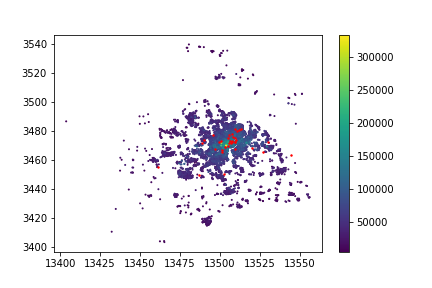
\includegraphics[width=.5\linewidth]{shanghai/shanghai.png}
  \caption{上海市住房价格分布} \label{fig:shanghai}
\end{figure}

其中横纵坐标单位为 \si{\kilo\metre}, 颜色的深浅反映了住房价格的高低, 红色标点表示区块中心所在位置.
使用前文所述的模型进行拟合, 得到结果如表 \ref{tab:shanghai_result} 所示.

使用拟合结果进行预测, 可以得到上海市的住房价格分布预测如图 \ref{fig:shanghai_predict} 所示.

\begin{figure}[htbp]
  \centering
  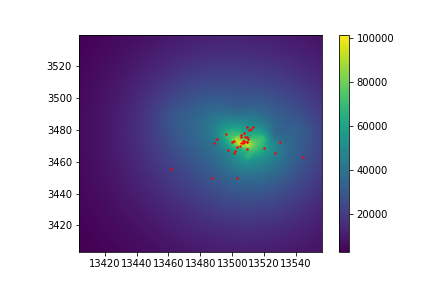
\includegraphics[width=.5\linewidth]{shanghai/shanghai_predict.png}
  \caption{上海市住房价格预测}
  \label{fig:shanghai_predict}
\end{figure}

进一步地, 对区块中心的类型进行统计分析可以得到上海市住房价格受教育, 医疗, 商业等因素的影响, 如图 \ref{fig:shanghai_impact}.
其中影响因子为正表示住房价格随与区位中心距离的缩短而提高.

\begin{figure}[htbp]
  \centering
  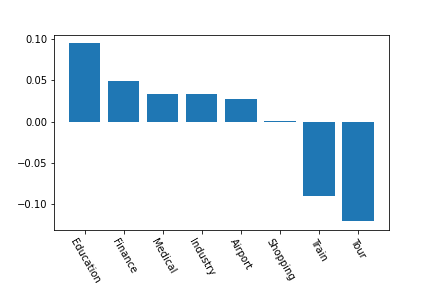
\includegraphics[width=.5\linewidth]{shanghai/shanghai_impact.png}
  \caption{上海市住房价格影响因子}
  \label{fig:shanghai_impact}
\end{figure}

% !TeX root = main.tex
\section{应用场景}
\subsection{消除信息不对称}
在房产市场中可能发生的一种情况是: 由于买方卖方的信息不对称而产生价格差额, 从而损害交易的健康性.
在本文提出的模型中, 只需给出目标房产的经纬度, 就可获得该房产的客观估值, 从而促进交易的公平性.

\subsection{房产估值}
已建成的房产价格在市场平衡中往往趋于稳定, 而在建工程的楼盘往往没有一个明确的报价, 本文的模型可用于在建工程的报价预测, 为广大消费者提供未来财产分配的合理建议.

% !TeX root = main.tex
\section{未来工作}
\subsection{模型选择}
受限于专业知识的不足, 笔者无法建立更加符合现实情况的模型进行统计.
目前人工智能发展迅速, 使用柔性更强的神经网络也许能够取得更好的结果.

此外, 由于北京, 上海的住房价格分布呈现明显的单中心性, 某地的住房价格很大程度上由其与市中心的距离决定, 这使得细部特征的研究较为困难.
如果能够使用统计学方法更加精确地提取细部特征, 则能够取得更好的效果.

除地理位置以外, 物业水平, 地方政策, 住房建成年限, 装修情况, 居民收入等也是影响房价的重要因素.
受限于数据来源的不足, 本研究暂未将其它因素纳入考虑范围.

\subsection{区位之间的相关性}
区位之间的相关性引起了本文主要的挑战, 在消除相关性后进行实验, 便能得到明确的区位比较.
在这里提出一个思路: 对区位进行进一步的细分, 到市中心的距离是一个重要因素, 那么与之相关的诸多因素, 例如商业, 餐饮, 可分为一类; 与到市中心距离关联不大的因素分为另一类: 例如景观等.

\subsection{密集数据}
本文的算法对世界各地的城市是通用的, 在获取一个城市的各主要区位分布, 房价分布后, 便能模拟出全城的房价分布, 因此可以尝试获取国外城市的类似数据, 例如可以从 Google Map 上收集城市的相关信息, 构建一个全球的房价分布.
在这个基础上, 我们可以进一步进行城市之间的比较——对比城市的系数组, 从而得到各个城市影响房价的主要区位条件, 这是研究世界文化, 经济差异的一个新思路.

% \subsection{数据清洗}
% 本研究所选取的北京住房价格数据来源于 2011 -- 2017 年的链家数据, 时间跨度大且较为老旧.
% 因此模型拟合的效果欠佳.
% 使用与 POI 数据同期的较新数据也许能够取得令人更加满意的结果.
% 拟合结果显示最小的特征值仅有 \num{1.86e-24}.
% 这意味着自变量, 即 $distance_i$ 之间很可能有较强的相关性.
% 而事实上也确实如此, 区位中心往往集中分布于城市中心, 从较大的尺度来看, 与区位中心的距离约等于与城市中心的距离, 因而具有强相关性.
% 可以考虑使用 Principal Component Analysis (PCA) 对自变量进行降维.

% !TeX root = main.tex
\section{总结}
在工程经济学的学习过程中, 我们在回归分析法的自学过程中产生了从区位视角, 运用模型分析房价的这样一种想法.

从眼就开始到结束的过程中, 我们的模型也发生了很大的变化.
一开始, 我们的研究方法是考虑一系列小区到某几个重要的区位点的距离 --- 如万象汇, 故宫博物院, 在拟合的过程中, 我们发现数据结果并不理想, 于是我们从前面提到的两篇硕士论文中寻找思路, 运用高德开放平台爬取大量 POI 点, 再利用模型进行分析.
一开始, 我们的模型算法也仅仅停留在最近点或是同类中心点距离的和, 由于 $R^2$ 较低, 我们不断调整算法, 最终使得 $R^2$ 达到比较好的水平, 同时这种算法对应的现实意义也是优于前两种的.

经过分析, 我们得到了价格热力图, 各个区位的影响因子, 并用这样的模型来估测 2018 与 2022 年的住房价格, 得到了比较好的结果.

其实, 这样的研究也是具有一定现实意义的.
正如老师在课堂上讲授的一样, 许多公共投资项目需要考虑其产生的社会总效益, 而房价正是反映人们对于某一建筑的支付意愿的一个窗口;同时, 这样的研究也可以为我们辅助我们预测房价.

土木学科叫做 Civil Engineering, 也就是民用工程.
这是一个与人的生活息息相关的学科, 实际地服务于社会, 服务于人们的日常生活, 是这个学科的终极意义, 这也是我们在工程经济学课上所体悟到的价值内核.


\bibliography{reference.bib}

\appendix
% % !TeX root = main.tex
\section{区位中心}
\subsection{上海市区位中心}
\begin{longtable}{cccc}
  \caption{上海市部分区位中心} \label{tab:shanghai_center}                             \\
  \toprule
  category  & name                   & longitude              & latitude               \\
  \midrule
  \endfirsthead
  \caption[]{上海市部分区位中心 (续)}                                                  \\
  \toprule
  category  & name                   & longitude              & latitude               \\
  \midrule
  \endhead
  \bottomrule
  \endfoot
  Industry  & 金桥经济技术开发区     & \tablenum{121.6786400} & \tablenum{31.22966585} \\
  Industry  & 松江出口加工区         & \tablenum{121.2935432} & \tablenum{31.02631179} \\
  Industry  & 上海嘉定工业园         & \tablenum{121.3724263} & \tablenum{31.27327714} \\
  Industry  & 上海张江高科产业园     & \tablenum{121.5879715} & \tablenum{31.19207597} \\
  Education & 复旦                   & \tablenum{121.5034418} & \tablenum{31.29818648} \\
  Education & 交大                   & \tablenum{121.4340058} & \tablenum{31.02657744} \\
  Education & 同济                   & \tablenum{121.4594209} & \tablenum{31.26880131} \\
  Education & 华师                   & \tablenum{121.4069147} & \tablenum{31.22928049} \\
  Education & 上外                   & \tablenum{121.4164398} & \tablenum{31.23557198} \\
  Education & 上财                   & \tablenum{121.4935940} & \tablenum{31.31111426} \\
  Shopping  & 南京路商业中心         & \tablenum{121.4748557} & \tablenum{31.23566243} \\
  Shopping  & 豫园商城商业中心       & \tablenum{121.4921009} & \tablenum{31.22692094} \\
  Shopping  & 徐家汇商业中心         & \tablenum{121.4372069} & \tablenum{31.19777322} \\
  Shopping  & 淮海中路商业中心       & \tablenum{121.4766402} & \tablenum{31.22570137} \\
  Shopping  & 五角场商业中心         & \tablenum{121.5149008} & \tablenum{31.30120284} \\
  Shopping  & 中山公园商业中心       & \tablenum{121.4782636} & \tablenum{31.27644059} \\
  Shopping  & 国际旅游度假区商业中心 & \tablenum{121.0634217} & \tablenum{31.07399471} \\
  Shopping  & 虹桥商务区商业中心     & \tablenum{121.3076676} & \tablenum{31.22221985} \\
  Medical   & 中山医院               & \tablenum{121.4585818} & \tablenum{31.22236830} \\
  Medical   & 瑞金医院               & \tablenum{121.4718929} & \tablenum{31.21922908} \\
  Medical   & 上海第九人民医院       & \tablenum{121.4941339} & \tablenum{31.25499654} \\
  Medical   & 仁济医院               & \tablenum{121.4805329} & \tablenum{31.25657087} \\
  Medical   & 华山医院               & \tablenum{121.4549848} & \tablenum{31.20442309} \\
  Medical   & 长海医院               & \tablenum{121.5259459} & \tablenum{31.31128891} \\
  Medical   & 长征医院               & \tablenum{121.4673474} & \tablenum{31.23425473} \\
  Medical   & 上海市第六人民医院     & \tablenum{121.4233709} & \tablenum{31.17804098} \\
  Airport   & 浦东                   & \tablenum{121.8082186} & \tablenum{31.14536056} \\
  Airport   & 虹桥                   & \tablenum{121.3205160} & \tablenum{31.24345821} \\
  Train     & 虹桥                   & \tablenum{121.3831639} & \tablenum{31.18216012} \\
  Train     & 上海南站               & \tablenum{121.4194368} & \tablenum{31.16319118} \\
  Train     & 上海火车站             & \tablenum{121.4564601} & \tablenum{31.25431173} \\
  Tour      & 城隍庙                 & \tablenum{121.4927642} & \tablenum{31.22552258} \\
  Tour      & 中华艺术宫             & \tablenum{121.4950264} & \tablenum{31.18643108} \\
  Tour      & 迪斯尼                 & \tablenum{121.6533616} & \tablenum{31.16663396} \\
  Finance   & 陆家嘴                 & \tablenum{121.5005196} & \tablenum{31.24288712} \\
\end{longtable}

% !TeX root = main.tex
\section{回归结果}
\subsection{上海市回归结果}
\begin{longtable}{lcccccc}
  \caption{Shanghai OLS Regression Results} \label{tab:shanghai_result}                                                                                      \\
  \toprule
                                  & \textbf{coef}      & \textbf{std err} & \textbf{t}         & \textbf{P$> |$t$|$} & \textbf{[0.025}   & \textbf{0.975]}   \\
  \midrule
  \endfirsthead
  \caption[]{Shanghai OLS Regression Results (续)}                                                                                                           \\
  \toprule
                                  & \textbf{coef}      & \textbf{std err} & \textbf{t}         & \textbf{P$> |$t$|$} & \textbf{[0.025}   & \textbf{0.975]}   \\
  \midrule
  \endhead
  \bottomrule
  \endfoot
  \textbf{Intercept}              & \tablenum{11.4569} & \tablenum{0.051} & \tablenum{225.186} & \tablenum{0.000}    & \tablenum{11.357} & \tablenum{11.557} \\
  \textbf{金桥经济技术开发区}     & \tablenum{-0.0051} & \tablenum{0.003} & \tablenum{-1.638}  & \tablenum{0.101}    & \tablenum{-0.011} & \tablenum{0.001}  \\
  \textbf{松江出口加工区}         & \tablenum{-0.0022} & \tablenum{0.001} & \tablenum{-1.490}  & \tablenum{0.136}    & \tablenum{-0.005} & \tablenum{0.001}  \\
  \textbf{上海嘉定工业园}         & \tablenum{0.0160}  & \tablenum{0.003} & \tablenum{4.593}   & \tablenum{0.000}    & \tablenum{0.009}  & \tablenum{0.023}  \\
  \textbf{上海张江高科产业园}     & \tablenum{-0.0422} & \tablenum{0.006} & \tablenum{-7.405}  & \tablenum{0.000}    & \tablenum{-0.053} & \tablenum{-0.031} \\
  \textbf{复旦}                   & \tablenum{-0.0694} & \tablenum{0.039} & \tablenum{-1.765}  & \tablenum{0.078}    & \tablenum{-0.146} & \tablenum{0.008}  \\
  \textbf{交大}                   & \tablenum{0.0166}  & \tablenum{0.001} & \tablenum{11.171}  & \tablenum{0.000}    & \tablenum{0.014}  & \tablenum{0.020}  \\
  \textbf{同济}                   & \tablenum{-0.0620} & \tablenum{0.020} & \tablenum{-3.178}  & \tablenum{0.001}    & \tablenum{-0.100} & \tablenum{-0.024} \\
  \textbf{华师}                   & \tablenum{0.0238}  & \tablenum{0.016} & \tablenum{1.505}   & \tablenum{0.132}    & \tablenum{-0.007} & \tablenum{0.055}  \\
  \textbf{上外}                   & \tablenum{-0.0133} & \tablenum{0.017} & \tablenum{-0.808}  & \tablenum{0.419}    & \tablenum{-0.046} & \tablenum{0.019}  \\
  \textbf{上财}                   & \tablenum{0.0095}  & \tablenum{0.012} & \tablenum{0.782}   & \tablenum{0.434}    & \tablenum{-0.014} & \tablenum{0.033}  \\
  \textbf{南京路商业中心}         & \tablenum{-0.0192} & \tablenum{0.084} & \tablenum{-0.228}  & \tablenum{0.820}    & \tablenum{-0.184} & \tablenum{0.146}  \\
  \textbf{豫园商城商业中心}       & \tablenum{-0.1499} & \tablenum{0.406} & \tablenum{-0.369}  & \tablenum{0.712}    & \tablenum{-0.946} & \tablenum{0.646}  \\
  \textbf{徐家汇商业中心}         & \tablenum{-0.1084} & \tablenum{0.016} & \tablenum{-6.677}  & \tablenum{0.000}    & \tablenum{-0.140} & \tablenum{-0.077} \\
  \textbf{淮海中路商业中心}       & \tablenum{0.2371}  & \tablenum{0.115} & \tablenum{2.054}   & \tablenum{0.040}    & \tablenum{0.011}  & \tablenum{0.463}  \\
  \textbf{五角场商业中心}         & \tablenum{-0.0040} & \tablenum{0.044} & \tablenum{-0.092}  & \tablenum{0.927}    & \tablenum{-0.090} & \tablenum{0.082}  \\
  \textbf{中山公园商业中心}       & \tablenum{0.0392}  & \tablenum{0.018} & \tablenum{2.178}   & \tablenum{0.029}    & \tablenum{0.004}  & \tablenum{0.074}  \\
  \textbf{国际旅游度假区商业中心} & \tablenum{-0.0101} & \tablenum{0.001} & \tablenum{-11.071} & \tablenum{0.000}    & \tablenum{-0.012} & \tablenum{-0.008} \\
  \textbf{虹桥商务区商业中心}     & \tablenum{0.0141}  & \tablenum{0.003} & \tablenum{5.306}   & \tablenum{0.000}    & \tablenum{0.009}  & \tablenum{0.019}  \\
  \textbf{中山医院}               & \tablenum{-0.1255} & \tablenum{0.029} & \tablenum{-4.371}  & \tablenum{0.000}    & \tablenum{-0.182} & \tablenum{-0.069} \\
  \textbf{瑞金医院}               & \tablenum{-0.0890} & \tablenum{0.068} & \tablenum{-1.315}  & \tablenum{0.188}    & \tablenum{-0.222} & \tablenum{0.044}  \\
  \textbf{上海第九人民医院}       & \tablenum{0.0877}  & \tablenum{0.040} & \tablenum{2.167}   & \tablenum{0.030}    & \tablenum{0.008}  & \tablenum{0.167}  \\
  \textbf{仁济医院}               & \tablenum{-0.0268} & \tablenum{0.034} & \tablenum{-0.800}  & \tablenum{0.424}    & \tablenum{-0.092} & \tablenum{0.039}  \\
  \textbf{华山医院}               & \tablenum{0.0894}  & \tablenum{0.018} & \tablenum{4.850}   & \tablenum{0.000}    & \tablenum{0.053}  & \tablenum{0.126}  \\
  \textbf{长海医院}               & \tablenum{0.0407}  & \tablenum{0.019} & \tablenum{2.120}   & \tablenum{0.034}    & \tablenum{0.003}  & \tablenum{0.078}  \\
  \textbf{长征医院}               & \tablenum{-0.0811} & \tablenum{0.067} & \tablenum{-1.206}  & \tablenum{0.228}    & \tablenum{-0.213} & \tablenum{0.051}  \\
  \textbf{上海市第六人民医院}     & \tablenum{0.0711}  & \tablenum{0.019} & \tablenum{3.720}   & \tablenum{0.000}    & \tablenum{0.034}  & \tablenum{0.109}  \\
  \textbf{浦东}                   & \tablenum{-0.0116} & \tablenum{0.002} & \tablenum{-6.800}  & \tablenum{0.000}    & \tablenum{-0.015} & \tablenum{-0.008} \\
  \textbf{虹桥[0]}                & \tablenum{-0.0155} & \tablenum{0.003} & \tablenum{-6.002}  & \tablenum{0.000}    & \tablenum{-0.021} & \tablenum{-0.010} \\
  \textbf{虹桥[1]}                & \tablenum{-0.0155} & \tablenum{0.003} & \tablenum{-6.002}  & \tablenum{0.000}    & \tablenum{-0.021} & \tablenum{-0.010} \\
  \textbf{上海南站}               & \tablenum{-0.0270} & \tablenum{0.012} & \tablenum{-2.215}  & \tablenum{0.027}    & \tablenum{-0.051} & \tablenum{-0.003} \\
  \textbf{上海火车站}             & \tablenum{0.1328}  & \tablenum{0.024} & \tablenum{5.649}   & \tablenum{0.000}    & \tablenum{0.087}  & \tablenum{0.179}  \\
  \textbf{城隍庙}                 & \tablenum{0.0241}  & \tablenum{0.365} & \tablenum{0.066}   & \tablenum{0.947}    & \tablenum{-0.691} & \tablenum{0.739}  \\
  \textbf{中华艺术宫}             & \tablenum{0.0571}  & \tablenum{0.008} & \tablenum{7.475}   & \tablenum{0.000}    & \tablenum{0.042}  & \tablenum{0.072}  \\
  \textbf{迪斯尼}                 & \tablenum{0.0397}  & \tablenum{0.006} & \tablenum{6.660}   & \tablenum{0.000}    & \tablenum{0.028}  & \tablenum{0.051}  \\
  \textbf{陆家嘴}                 & \tablenum{-0.0494} & \tablenum{0.042} & \tablenum{-1.172}  & \tablenum{0.241}    & \tablenum{-0.132} & \tablenum{0.033}  \\
\end{longtable}


\section{成员分工}
\begin{description}
  \item[李钦] 摘要, 引言, 模型选择, POI 数据爬取, 回归计算与样本估测
  \item[李泽宇] 数据分析, 模型评价, 应用场景, 未来工作
  \item[陈奕玮] 引言, 相关工作, 数据来源, 总结
\end{description}

\end{document}
